% main1.tex -- H-main.  Section 1: the problem and the answer.
%======================================================================
\section{The problem and the answer}\label{sec:intro}
%======================================================================

Harry stands at the origin of the plane. Somewhere on the circle of radius $d$ around him hovers the Snitch, a small
golden ball; Harry knows $d$ but not the direction. The Snitch is shy: at every moment it flies with speed $v$
straight away from Harry, wherever he is. Harry runs with speed at most $1$, and he sees the Snitch as soon as it is
within distance $\varepsilon$ of him. He cannot see it before that, so he gets no information along the way, and he must
fix his whole route in advance. Can he plan a route that finds the Snitch whatever its starting direction, and can he do
so in a time that does not blow up as his eyesight $\varepsilon$ gets worse and worse?

\textbf{The problem.} Identify $\R^2$ with $\C$. A \emph{pursuer path} is a $1$-Lipschitz map $H:[0,\infty)\to\R^2$
with $H(0)=0$. For a direction $\alpha\in[0,2\pi)$ the Snitch $S_\alpha$ starts at $de^{i\alpha}$ and moves by
\begin{equation}\label{eq:snitch}
S'_\alpha(t) = v\,\frac{S_\alpha(t)-H(t)}{|S_\alpha(t)-H(t)|},\qquad S_\alpha(0)=de^{i\alpha},
\end{equation}
where $0<v<1$. Since $H$ may not depend on $\alpha$, Harry has to deal with all directions at once; we call $S_\alpha$
the \emph{candidate} with direction $\alpha$. The right-hand side of \eqref{eq:snitch} is continuous in $t$ and locally
Lipschitz in $S$ away from $H(t)$, so each candidate exists up to the first time it meets $H$; it has a limit there,
because $|S'_\alpha|=v$. Candidate $\alpha$ is \emph{caught} if $S_\alpha(t)=H(t)$ for some $t$, and \emph{seen} (with
vision radius $\varepsilon\in[0,d)$) if $|S_\alpha(t)-H(t)|\le\varepsilon$ for some $t$ in its interval of existence or
at its end. Equation \eqref{eq:snitch} does not change under $(S,H,t)\mapsto(\lambda S,\lambda H,\lambda t)$, so we may
and often will take $d=1$.

\begin{figure}[!htbp]
\centering
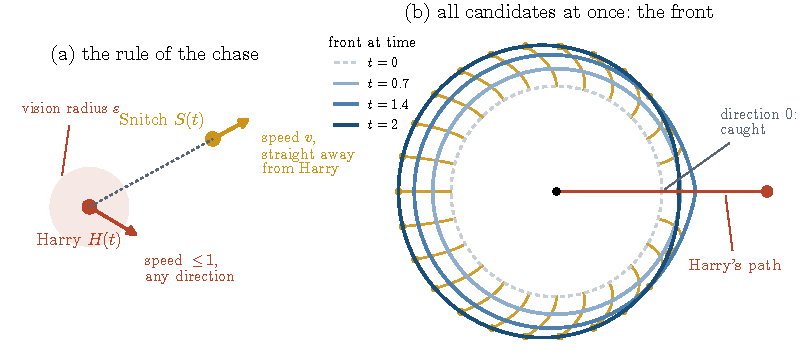
\includegraphics[width=\linewidth]{figs/fig_problem.pdf}
\caption{(a) The rule: the Snitch always flees straight away from Harry. (b) Harry does not know where the Snitch
started, so he faces one candidate for each direction (gold tracks, here while Harry runs straight to the right, with
the exaggerated speed $v=0.25$). Together the candidates form a closed curve, the \emph{front}, which swells and bends
as Harry moves. The fronts shown are those of the regularised candidates of Section~\ref{sec:virtual} (with
$\varepsilon=0.04$), which pass smoothly through direction~$0$; the front of the true candidates has a hole there,
because candidate~$0$ is caught.}
\label{fig:problem}
\end{figure}

\textbf{An easy case, and the real difficulty.} If $(1+2\pi)v\le\varepsilon/d$, Harry simply runs to the circle and once
around it: he passes the starting point of each candidate before time $(1+2\pi)d$, when that candidate has moved less
than $(1+2\pi)vd\le\varepsilon$, so he sees it. This argument says nothing when $\varepsilon$ is small compared with
$v$, and that is the interesting regime: we want a speed range for the Snitch, and a search time, that do not depend on
$\varepsilon$ at all. If that is possible, a limiting argument even lets Harry \emph{catch} the Snitch ($\varepsilon=0$).

\begin{theorem}[Uniform-in-$\varepsilon$ search]\label{thm:main}
There exist absolute constants $v_0>0$, $T_0>0$ and $\varepsilon_*>0$ such that for every $d>0$, every
$\varepsilon\in(0,d)$ and every $v\in(0,v_0]$ the explicit path $H=H_{v,\varepsilon,d}$ --- Design~T
\textup{(Definition~\ref{def:designT})} followed by the greedy chase \textup{(Definition~\ref{def:chase})} on the
working front of Theorem~\ref{thm:touchdown}, both run at vision radius $\varepsilon':=\min(\varepsilon,\varepsilon_*d)$
and scaled by $d$ --- satisfies $H(0)=0$, $|H'|\le1$ a.e., and for every $\alpha\in[0,2\pi)$ there is $t\le T_0d$
with $|S_\alpha(t)-H(t)|\le\varepsilon$.
\end{theorem}

\begin{corollary}[Exact catch]\label{cor:exact}
For every $d>0$ and $v\in(0,v_0]$ there is a $1$-Lipschitz path $H$ with $H(0)=0$ such that for every
$\alpha\in[0,2\pi)$ there is $t\le T_0d$ with $S_\alpha(t)=H(t)$.
\end{corollary}

The theorem is proved at the end of Section~\ref{sec:assembly} (any $T_0\ge15$ works), the corollary in
Section~\ref{sec:exact}. We do not try to make $v_0$ explicit: it is ``small enough that finitely many error terms of
size $O(v)$ fit under fixed margins''. A companion paper with the same architecture \cite{short} tracks every constant
and obtains $v_0=5.8\cdot10^{-3}$ and $T_0=13.1$, at the price of about fifty pages and one computer-checked constant.
Simulations (such as Figure~\ref{fig:designT}, where $v=0.1$) suggest that the same path works for much larger $v$.

\textbf{How the proof goes.} The candidates form a closed curve, the \emph{front}; Harry sees a candidate when he comes
within $\varepsilon$ of its point on the front. So Harry must sweep a curve whose points run away from him. Our path
(Section~\ref{sec:idea}) has two parts. \emph{Design~T}: Harry runs straight through the front, then turns and runs
along a straight line that just grazes the rest of it. \emph{The walk}: from the grazing point he walks along the
front in short straight legs, each aimed at the point an arclength $\varepsilon$ further on, and sees everything he
passes. The walk takes a bounded time provided the front stays nearly straight on every scale between $\varepsilon$
and a fixed length, and the heart of the proof is a bootstrap showing exactly this (Section~\ref{sec:chase}). It is
measured by the \emph{bendiness} of a pair of points, arclength minus chord (Section~\ref{sec:virtual}). The bootstrap
needs good starting data, which the grazing touch-down provides (Section~\ref{sec:touchdown}). One end of the front is
left close behind Harry at touch-down; we show that it stays straight while he walks away from it
(Section~\ref{sec:assembly}). Finally the time bound does not depend on $\varepsilon$, so we can let $\varepsilon\to0$
(Section~\ref{sec:exact}).

The main text states every result and proves the short ones. The three long arguments are in the appendices: the
bootstrap (Appendix~A), the shape of the front at touch-down (Appendix~B), and the departure from the tail end together
with the assembly (Appendix~C).

\textbf{Notation.} For $a,b\in\R^2=\C$: $a\cdot b:=\operatorname{Re}(\bar ab)$, $a\times b:=\operatorname{Im}(\bar ab)$
and $a^\perp:=ia$, so that $a^\perp\cdot b=a\times b$. We write $\mu:=v/(1-v)$ and $\mu_T:=3v/(1+v)$ (both are
$O(v)$; $\mu_T$ is the small loss in the flatness exponent of the front at touch-down, Theorem~\ref{thm:touchdown}).
From Section~\ref{sec:virtual} on, $d=1$ (except in the scaling step at the end of Section~\ref{sec:assembly}).
Throughout, $C,c$ denote positive constants that depend only on the locked numbers below (and on the absolute constants
of Theorem~\ref{thm:touchdown}), never on $R$, $v$ or $\varepsilon$; dependence on $R$ is written explicitly, as in
$O_R(v)$ (a quantity bounded by $C(R)\,v$).

\takeaway{Locked numbers}{%
The proof uses a handful of fixed numbers. Nothing depends on getting them optimal; they are fixed once and for all so
that no choice depends on a later one. With their roles (made precise where they are used):
$\gamma:=\frac23$ (flatness exponent of the walk), $\gamma_D:=\frac34$ (the same on its first stretch),
$\nu:=\frac1{24}$ (exponent of a weight that absorbs a logarithm), $\kappa:=\frac54$ (allowed stretch of a pair),
$c_A:=\frac12$ (allowed shortening of chords), $K_f:=10$ (near/far threshold, in pair lengths), $K_R:=12$ (cap on gaps,
in units of $R$), $c_{\mathrm{off}}:=\frac12$ (offset threshold for far pairs, in units of $R$), $K_\varepsilon:=10$
($\varepsilon\le R/K_\varepsilon$), $d_L:=2$ (a leg lasts at most $d_L\varepsilon$), $\delta_1:=\frac54$ (stretch factor
during one leg), $s_0:=\frac18$ (start bendiness), $A_0:=2$ (amplification allowed for far pairs), $f_F:=\frac12$
(bendiness of far pairs), and $m:=\frac1{10}$ (size of the bendiness bound).
Four more scales are chosen later, in the strict order $\lambda_0\to R\to v_0\to\varepsilon_*$: a scale $\lambda_0$
below which the front at touch-down is known to be flat (Section~\ref{sec:touchdown}), a small length $R$ up to which
the walk controls the bendiness, the speed threshold $v_0$, and the threshold $\varepsilon_*$ for the vision radius.
The precise conditions, the \emph{Parameter Lock}, are stated in Section~\ref{sec:assembly}, where all the objects they
refer to have been defined.}

